% --- SECTION: NeRFs ---
\section{Trường bức xạ nơ-ron} \label{sec:nerfs}

Trong phần này, luận văn sẽ trình bày chi tiết về Trường bức xạ nơ-ron (NeRF) \cite{Mildenhall2020NeRF}, một phương pháp tiên tiến để biểu diễn và tái tạo các cảnh 3D phức tạp nhằm mục đích tổng hợp góc nhìn mới với chất lượng quang học chân thực, cũng như được sử dụng để tái tạo đám mây điểm 3D với độ chi tiết cao. Phần này sẽ giới thiệu về phương pháp biểu diễn hình dạng 3D bằng mạng nơ-ron và các kỹ thuật tổng hợp góc nhìn mới, sau đó đi sâu vào cách NeRF biểu diễn cảnh, cách cơ chế kết xuất thể tích được mô tả ở mục  \ref{subsec:volume_rendering_detailed} được sử dụng, và cuối cùng là quy trình tối ưu hóa mạng NeRF.

% % --- SUBSECTION: Neural 3D shape representations ---
% \subsection{Các phương pháp biểu diễn hình dạng 3D bằng mạng nơ-ron} \label{subsec:neural_shape_repr}

% Một hướng nghiên cứu nổi bật trong thị giác máy tính là sử dụng trọng số của mạng nơ-ron Perceptron Đa lớp (MLP) để mã hóa các đối tượng và cảnh 3D, thay thế các biểu diễn rời rạc truyền thống như lưới tam giác hoặc lưới voxel \cite{Mildenhall2020NeRF}. Các mạng này thường ánh xạ trực tiếp từ tọa độ không gian 3D, $\mathbf{x} = (x, y, z)$, sang một biểu diễn hình học ẩn tại điểm đó. Các nghiên cứu ban đầu tập trung vào biểu diễn hình dạng 3D liên tục bằng cách huấn luyện mạng nơ-ron để ánh xạ tọa độ 3D thành Hàm khoảng cách có dấu (SDF) \cite{Park19DeepSDF, Jiang20Local} hoặc Trường chiếm dụng \cite{Mescheder19Occupancy, Genova20Local}. Tuy nhiên, những phương pháp này thường yêu cầu dữ liệu hình học 3D thực, vốn khó thu thập trong các ứng dụng thực tế. Để khắc phục, các nghiên cứu sau này phát triển các phương pháp kết xuất khả vi, cho phép tối ưu hóa biểu diễn hình dạng ẩn chỉ từ hình ảnh 2D. Chẳng hạn, một số công trình biểu diễn bề mặt thông qua trường chiếm dụng 3D và sử dụng phương pháp giao điểm tia để xác định bề mặt đối tượng, sau đó tính đạo hàm thông qua kỹ thuật kết xuất khả vi \cite{Niemeyer19Differentiable}. Các phương pháp khác đề xuất biểu diễn 3D bằng mạng nơ-ron trả về vector đặc trưng và màu RGB tại mỗi tọa độ 3D, kết hợp với hàm kết xuất khả vi để xác định vị trí bề mặt dọc theo tia nhìn \cite{Sitzmann19SRN}. Mặc dù các kỹ thuật này có khả năng biểu diễn hình học phức tạp với độ phân giải cao, chúng thường bị giới hạn ở các hình dạng đơn giản và dễ tạo ra kết quả kết xuất bị làm mịn quá mức.

% Trong bối cảnh đó, mô hình Trường bức xạ nơ-ron (NeRF) đề xuất một chiến lược thay thế bằng cách tối ưu hóa mạng nơ-ron để mã hóa trực tiếp trường bức xạ 5D, biểu diễn đồng thời hình học và ngoại hình của đối tượng với độ chi tiết cao. Nhờ vậy, NeRF cho phép kết xuất các góc nhìn mới một cách chân thực, ngay cả đối với các cảnh 3D phức tạp \cite{Mildenhall2020NeRF}.

\subsection{Biểu diễn cảnh bằng trường bức xạ nơ-ron} \label{subsec:nerf_representation}

NeRF biểu diễn một cảnh tĩnh liên tục dưới dạng trường bức xạ 5D, ánh xạ tọa độ 5D gồm vị trí không gian 3D \(\mathbf{x} = (x, y, z)\) và vector hướng nhìn 3D \(\mathbf{d}\) (thường là vector đơn vị) tới màu sắc \(\mathbf{c} = (r, g, b)\) và mật độ \(\sigma\) tại điểm đó. Thay vì biểu diễn trường 5D này một cách rõ ràng, NeRF xấp xỉ nó bằng một mạng MLP \(F_{\Theta}: (\mathbf{x}, \mathbf{d}) \to (\mathbf{c}, \sigma)\), với \(\Theta\) là các trọng số của mạng \cite{Mildenhall2020NeRF}.

\begin{figure}[H]
    \centering
    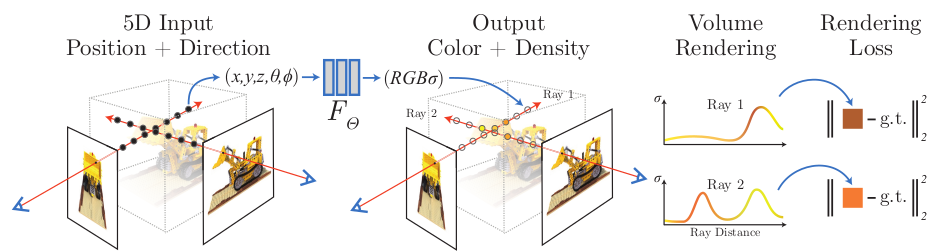
\includegraphics[width=\linewidth]{figures/c3/nerf.png}
    \caption{Kiến trúc mạng Trường bức xạ nơ-ron \cite[Fig.~2]{Mildenhall2020NeRF}.}
    \label{fig:nerf}
\end{figure}

Để đảm bảo tính nhất quán đa góc nhìn, kiến trúc mạng NeRF được minh họa ở Hình \ref{fig:nerf} được thiết kế sao cho mật độ \(\sigma\) chỉ phụ thuộc vào vị trí \(\mathbf{x}\), trong khi màu sắc \(\mathbf{c}\) phụ thuộc vào cả \(\mathbf{x}\) và \(\mathbf{d}\). Điều này phản ánh rằng mật độ (biểu thị hình học và vật liệu) không thay đổi theo hướng nhìn, nhưng màu sắc có thể thay đổi do các hiệu ứng chiếu sáng, phản xạ \cite{Mildenhall2020NeRF}.

Cụ thể, MLP \(F_{\Theta}\) xử lý tọa độ \(\mathbf{x}\) qua 8 lớp kết nối đầy đủ, mỗi lớp có 256 kênh và sử dụng hàm kích hoạt ReLU. Đầu ra của khối này gồm giá trị mật độ \(\sigma\) và một vector đặc trưng 256 chiều. Vector đặc trưng này được kết hợp với thông tin hướng nhìn \(\mathbf{d}\) và đưa qua một lớp kết nối đầy đủ (128 kênh, hàm ReLU) để dự đoán màu sắc \(\mathbf{c}\). Việc sử dụng \(\mathbf{d}\) cho phép NeRF mô phỏng các hiệu ứng thay đổi cường độ sáng, phản xạ, điều mà các mô hình chỉ dựa vào tọa độ điểm \(\mathbf{x}\) khó thực hiện.

% % --- SUBSECTION: Volume Rendering with Radiance Fields ---
% \subsection{Kết xuất thể tích với Trường bức xạ} \label{subsec:volume_rendering}

% Với biểu diễn cảnh 5D dưới dạng mật độ thể tích $\sigma(\mathbf{x})$ và bức xạ $\mathbf{c}(\mathbf{x}, \mathbf{d})$ tại mọi điểm trong không gian, NeRF sử dụng nguyên lý từ kỹ thuật kết xuất thể tích cổ điển \ref{subsec:volume_rendering_detailed}
% để tính toán màu sắc của một tia từ vị trí, hướng máy ảnh bất kỳ đi xuyên qua cảnh.

% Mật độ thể tích $\sigma(\mathbf{x})$ tại một vị trí $\mathbf{x}$ có thể được diễn giải như là xác suất vi phân mà một tia sáng kết thúc (bị hấp thụ hoặc tán xạ) tại một hạt vô cùng nhỏ ở vị trí đó. Màu sắc kỳ vọng $C(\mathbf{r})$ của một tia máy ảnh $\mathbf{r}(t) = \mathbf{o} + t\mathbf{d}$ (với $\mathbf{o}$ là gốc và $\mathbf{d}$ là hướng của tia) đi từ giới hạn gần $t_n$ đến giới hạn xa $t_f$ được tính bằng tích phân:
% \begin{equation} \label{eq:volume_rendering_integral}
% C(\mathbf{r}) = \int_{t_n}^{t_f} T(t) \sigma(\mathbf{r}(t)) \mathbf{c}(\mathbf{r}(t), \mathbf{d}) dt,
% \end{equation}
% trong đó hàm $T(t)$ biểu thị độ truyền qua tích lũy dọc theo tia từ $t_n$ đến $t$:
% \begin{equation} \label{eq:transmittance}
% T(t) = \exp\left(-\int_{t_n}^{t} \sigma(\mathbf{r}(s)) ds\right).
% \end{equation}
% $T(t)$ đại diện cho xác suất mà tia sáng có thể đi từ $t_n$ đến $t$ mà không va chạm vào bất kỳ hạt nào khác trong môi trường. Việc kết xuất một góc nhìn mới từ NeRF đòi hỏi phải ước lượng tích phân $C(\mathbf{r})$ này cho mỗi tia máy ảnh đi qua từng điểm ảnh.

% Vì hàm biểu diễn cảnh là liên tục và được định nghĩa bởi mạng nơ-ron, tích phân trong Phương trình \eqref{eq:volume_rendering_integral} không thể tính chính xác một cách giải tích. Do đó, NeRF sử dụng phương pháp cầu phương số (numerical quadrature) để xấp xỉ tích phân này. Thay vì sử dụng cầu phương xác định (deterministic quadrature) như thường làm với lưới voxel rời rạc (điều này sẽ giới hạn độ phân giải của biểu diễn liên tục), NeRF áp dụng kỹ thuật **lấy mẫu phân tầng (stratified sampling)**. Khoảng $[t_n, t_f]$ dọc theo tia được chia thành $N$ khoảng con (bins) đều nhau. Sau đó, một mẫu $t_i$ được rút ngẫu nhiên và đều từ bên trong mỗi khoảng con thứ $i$:
% \begin{equation} \label{eq:stratified_sampling}
% t_i \sim \mathcal{U}\left[t_n + \frac{i-1}{N}(t_f - t_n), t_n + \frac{i}{N}(t_f - t_n)\right].
% \end{equation}
% Mặc dù chỉ sử dụng một tập hợp hữu hạn các mẫu, việc lấy mẫu phân tầng đảm bảo rằng mạng MLP được truy vấn tại các vị trí liên tục dọc theo tia trong suốt quá trình tối ưu hóa, cho phép học được biểu diễn liên tục của cảnh [731].

% Với tập hợp các mẫu $\{t_i\}$, màu sắc của tia $\mathbf{r}$ được ước lượng bằng quy tắc cầu phương dựa trên công trình của Max \cite{Max95Optical}
% , tương tự như phép tổng hợp alpha (alpha compositing) \cite{porter1984compositing}: % Thay bằng key BibTeX
% \begin{equation} \label{eq:volume_rendering_discrete}
% \hat{C}(\mathbf{r}) = \sum_{i=1}^{N} T_i (1 - \exp(-\sigma_i \delta_i)) \mathbf{c}_i,
% \end{equation}
% trong đó $\delta_i = t_{i+1} - t_i$ là khoảng cách giữa các mẫu liền kề, $\sigma_i = \sigma(\mathbf{r}(t_i))$ và $\mathbf{c}_i = \mathbf{c}(\mathbf{r}(t_i), \mathbf{d})$ là mật độ và màu sắc được dự đoán bởi mạng $F_\Theta$ tại mẫu thứ $i$. Độ truyền qua tích lũy $T_i$ được tính rời rạc:
% \begin{equation} \label{eq:transmittance_discrete}
% T_i = \exp\left(-\sum_{j=1}^{i-1} \sigma_j \delta_j\right).
% \end{equation}
% Hệ số $(1 - \exp(-\sigma_i \delta_i))$ chính là giá trị alpha $\alpha_i$, đại diện cho độ chắn sáng (opacity) của đoạn $\delta_i$. Quan trọng là, hàm ước lượng màu $\hat{C}(\mathbf{r})$ theo công thức \eqref{eq:volume_rendering_discrete} là hoàn toàn khả vi (differentiable) đối với các đầu ra $(\sigma_i, \mathbf{c}_i)$ của mạng nơ-ron, cho phép lan truyền ngược gradient trong quá trình tối ưu hóa [732, 733].

% % --- SUBSECTION: Optimizing a Neural Radiance Field ---
% \subsection{Tối ưu hóa Trường bức xạ nơ-ron} \label{subsec:optimizing_nerf}

% Mặc dù các thành phần cốt lõi để biểu diễn cảnh và kết xuất góc nhìn mới bằng NeRF đã được mô tả, nhóm tác giả NeRF nhận thấy rằng chỉ những thành phần này là chưa đủ để đạt được chất lượng kết xuất hàng đầu cho các cảnh phức tạp [737, 738]. Do đó, họ đã giới thiệu hai cải tiến quan trọng để cho phép biểu diễn hiệu quả các cảnh có độ phân giải cao: **Mã hóa vị trí (Positional Encoding)** cho tọa độ đầu vào và **Quy trình lấy mẫu phân cấp (Hierarchical Volume Sampling)** [739].


% % --- SUBSUBSECTION: Hierarchical Volume Sampling ---
% \subsubsection{Lấy mẫu thể tích phân cấp (Hierarchical Volume Sampling)} \label{subsubsec:hierarchical_sampling}

% Chiến lược kết xuất bằng cách truy vấn mạng NeRF tại $N$ điểm lấy mẫu dày đặc dọc theo mỗi tia máy ảnh (như mô tả ở Mục \ref{subsec:volume_rendering}) là không hiệu quả về mặt tính toán. Các vùng không gian trống hoặc bị che khuất, không đóng góp vào màu sắc cuối cùng của pixel, vẫn bị lấy mẫu lặp đi lặp lại [753]. Lấy cảm hứng từ các công trình ban đầu về kết xuất thể tích \cite{Levoy90Efficient},
% NeRF đề xuất một chiến lược **lấy mẫu phân cấp (hierarchical sampling)** để tăng hiệu quả kết xuất bằng cách phân bổ các mẫu tỷ lệ thuận với đóng góp dự kiến của chúng vào kết quả cuối cùng [754].

% Thay vì chỉ sử dụng một mạng duy nhất, NeRF tối ưu hóa đồng thời hai mạng: một mạng "thô" ("coarse" network) và một mạng "tinh" ("fine" network) [755]. Quy trình hoạt động như sau:
% \begin{enumerate}
%     \item Lấy mẫu một tập hợp $N_c$ vị trí dọc theo tia bằng phương pháp lấy mẫu phân tầng (Stratified Sampling - Phương trình \eqref{eq:stratified_sampling}).
%     \item Truy vấn mạng "thô" tại $N_c$ vị trí này để có được tập các cặp $(\mathbf{c}_{c,i}, \sigma_{c,i})$.
%     \item Tính toán màu sắc ước lượng $\hat{C}_c(\mathbf{r})$ từ mạng thô bằng công thức \eqref{eq:volume_rendering_discrete}.
%     \item Dựa trên kết quả của mạng thô, tạo ra một hàm mật độ xác suất (PDF) rời rạc dọc theo tia, thiên vị về các vùng có khả năng chứa nội dung nhìn thấy được. Cụ thể, viết lại $\hat{C}_c(\mathbf{r})$ dưới dạng tổng có trọng số của các màu mẫu:
%         \begin{equation} \label{eq:hierarchical_weights}
%         \hat{C}_c(\mathbf{r}) = \sum_{i=1}^{N_c} w_i \mathbf{c}_{c,i}, \quad \text{với} \quad w_i = T_i (1 - \exp(-\sigma_{c,i} \delta_i)).
%         \end{equation}
%     Sau đó, chuẩn hóa các trọng số $w_i$ để tạo thành PDF: $\hat{w}_i = w_i / \sum_{j=1}^{N_c} w_j$ [758-760].
%     \item Rút $N_f$ mẫu vị trí thứ hai từ PDF này bằng phương pháp lấy mẫu biến đổi ngược (inverse transform sampling) [761].
%     \item Truy vấn mạng "tinh" tại tất cả $N_c + N_f$ mẫu (bao gồm cả mẫu từ bước 1 và bước 5).
%     \item Tính toán màu sắc cuối cùng $\hat{C}_f(\mathbf{r})$ bằng công thức \eqref{eq:volume_rendering_discrete} nhưng sử dụng $N_c + N_f$ mẫu và các giá trị $(\mathbf{c}_{f,i}, \sigma_{f,i})$ từ mạng tinh [761, 762].
% \end{enumerate}
% Quy trình này giúp tập trung năng lực tính toán vào các vùng không gian quan trọng, tương tự như ý tưởng của lấy mẫu theo tầm quan trọng (importance sampling), nhưng NeRF sử dụng các mẫu này để tạo ra một sự rời rạc hóa không đều của toàn bộ miền tích phân thay vì coi mỗi mẫu là một ước lượng xác suất độc lập cho toàn bộ tích phân.

% --- SUBSECTION: Volume Rendering with Radiance Fields ---
\subsection{Kết xuất thể tích với Trường bức xạ} \label{subsec:volume_rendering}

Kết xuất thể tích là một kỹ thuật cốt lõi trong phương pháp Trường bức xạ nơ-ron (NeRF), cho phép biểu diễn và tái tạo hình ảnh từ các trường bức xạ 5D liên tục. Trong NeRF, một cảnh được biểu diễn dưới dạng một hàm liên tục ánh xạ từ tọa độ không gian 3D $\mathbf{x} = (x, y, z)$ và hướng nhìn 2D $\mathbf{d} = (\theta, \phi)$ (thường được biểu diễn dưới dạng vector đơn vị 3D) đến mật độ thể tích $\sigma$ và màu sắc phát xạ phụ thuộc hướng nhìn $\mathbf{c}(\mathbf{x}, \mathbf{d}) = (r, g, b)$\cite{Mildenhall2020NeRF}. Quá trình kết xuất sử dụng các nguyên tắc của kết xuất thể tích cổ điển để tính màu sắc của một tia máy ảnh đi qua cảnh.

Màu sắc kỳ vọng $C(\mathbf{r})$ của một tia máy ảnh $\mathbf{r}(t) = \mathbf{o} + t \mathbf{d}$, với $\mathbf{o}$ là điểm xuất phát của tia, $\mathbf{d}$ là hướng tia, và $t$ nằm trong khoảng giới hạn gần và xa $[t_n, t_f]$, được tính bằng tích phân sau:

\begin{equation}
C(\mathbf{r}) = \int_{t_n}^{t_f} T(t) \sigma(\mathbf{r}(t)) \mathbf{c}(\mathbf{r}(t), \mathbf{d}) \, dt,
\end{equation}
trong đó $T(t)$ là độ truyền qua tích lũy, được định nghĩa như:

\begin{equation}\label{do_truyen_qua}
T(t) = \exp\left(-\int_{t_n}^{t} \sigma(\mathbf{r}(s)) \, ds\right).
\end{equation}

Hàm $T(t)$ biểu thị xác suất mà tia đi từ $t_n$ đến $t$ mà không va chạm với bất kỳ hạt nào, tức là xác suất tia không bị chặn. Mật độ thể tích $\sigma(\mathbf{r}(t))$ được xem như xác suất vi phân của việc tia bị chấm dứt tại vị trí $\mathbf{r}(t)$, và $\mathbf{c}(\mathbf{r}(t))$.

Để ước lượng số tích phân liên tục này, NeRF sử dụng phương pháp lấy mẫu phân tầng. Khoảng $[t_n, t_f]$ được chia thành $N$ đoạn đều nhau, và một mẫu được rút ngẫu nhiên từ mỗi đoạn:

\begin{equation}
t_i \sim \mathcal{U}\left[t_n + \frac{i-1}{N}(t_f - t_n), t_n + \frac{i}{N}(t_f - t_n)\right].
\end{equation}

Phương pháp này cho phép biểu diễn cảnh liên tục, vì mạng nơ-ron được truy vấn tại các vị trí liên tục trong suốt quá trình tối ưu hóa. Màu sắc được ước lượng bằng quy tắc xấp xỉ tích phân:

\begin{equation}\label{color_cumulative}
\hat{C}(\mathbf{r}) = \sum_{i=1}^N T_i \left(1 - \exp(-\sigma_i \delta_i)\right) \mathbf{c}_i,
\end{equation}
trong đó $T_i = \exp\left(-\sum_{j=1}^{i-1} \sigma_j \delta_j\right)$, và $\delta_i = t_{i+1} - t_i$ là khoảng cách giữa các mẫu liền kề. Công thức \ref{color_cumulative} tương đương với phép tổng hợp alpha truyền thống với $\alpha_i = 1 - \exp(-\sigma_i \delta_i)$, đảm bảo hàm kết xuất là khả vi, cho phép tối ưu hóa dựa trên gradient.

\subsection{Tối ưu hóa Trường bức xạ nơ-ron} \label{subsec:optimizing_nerf}

Việc tối ưu hóa NeRF bao gồm việc điều chỉnh các tham số $\Theta$ của mạng MLP $F_\Theta: (\mathbf{x}, \mathbf{d}) \to (\mathbf{c}, \sigma)$ để giảm thiểu sai số giữa các hình ảnh quan sát và các hình ảnh được kết xuất từ biểu diễn trường bức xạ. Quá trình này sử dụng giảm gradient với hàm mất mát là tổng bình phương sai số giữa màu sắc dự đoán và màu sắc thực tế:

\begin{equation}
\mathcal{L} = \sum_{\mathbf{r} \in \mathcal{R}} \left[ \left\| \hat{C}_c(\mathbf{r}) - C(\mathbf{r}) \right\|_2^2 + \left\| \hat{C}_f(\mathbf{r}) - C(\mathbf{r}) \right\|_2^2 \right],
\end{equation}
trong đó $\mathcal{R}$ là tập hợp các tia trong mỗi lô, $\hat{C}_c(\mathbf{r})$ và $\hat{C}_f(\mathbf{r})$ lần lượt là màu sắc dự đoán từ mạng thô và mạng tinh, và $C(\mathbf{r})$ là màu sắc thực tế. Hàm mất mát này khuyến khích mạng dự đoán mật độ thể tích cao và màu sắc chính xác tại các vị trí chứa nội dung cảnh thực.

Để cải thiện hiệu suất, NeRF sử dụng mã hóa vị trí để ánh xạ tọa độ đầu vào vào không gian chiều cao hơn giúp mạng học đặc trưng về vị trí trong không gian tốt hơn. Hàm mã hóa vị trí $\gamma(p)$ được định nghĩa như:

\begin{equation}
\gamma(p) = \left( \sin(2^0 \pi p), \cos(2^0 \pi p), \ldots, \sin(2^{L-1} \pi p), \cos(2^{L-1} \pi p) \right),
\end{equation}
với $L=10$ cho tọa độ không gian $\mathbf{x}$ và $L=4$ cho hướng nhìn $\mathbf{d}$. Hàm này được áp dụng riêng cho mỗi thành phần của $\mathbf{x}$ và $\mathbf{d}$, sau khi được chuẩn hóa về $[-1, 1]$. Mã hóa vị trí cải thiện đáng kể khả năng biểu diễn chi tiết hình học và màu sắc của mô hình.

Ngoài ra, NeRF sử dụng một quy trình lấy mẫu phân cấp (xem Mục \ref{subsubsec:hierarchical_sampling}) để phân bổ hiệu quả các mẫu vào các vùng có nội dung cảnh quan trọng.

\subsection{Lấy mẫu phân cấp} \label{subsubsec:hierarchical_sampling}

Lấy mẫu phân cấp là một cải tiến quan trọng trong NeRF để tăng hiệu quả kết xuất bằng cách phân bổ các mẫu một cách thông minh vào các vùng có khả năng chứa nội dung cảnh hữu ích. Thay vì chỉ sử dụng một mạng duy nhất, NeRF tối ưu hóa đồng thời hai mạng: một mạng "thô" và một mạng "tinh".

Đầu tiên, $N_c$ điểm được lấy mẫu bằng phương pháp phân tầng và được đánh giá bởi mạng thô. Kết quả từ mạng thô được sử dụng để tạo ra một phân phối xác suất dọc theo tia, dựa trên trọng số của các mẫu:

\begin{equation}
\hat{C}_c(\mathbf{r}) = \sum_{i=1}^{N_c} w_i \mathbf{c}_i, \quad w_i = T_i \left(1 - \exp(-\sigma_i \delta_i)\right),
\end{equation}
trong đó $w_i$ là trọng số của mẫu thứ $i$, và $T_i$ được tính như trong công thức \ref{do_truyen_qua}. Các trọng số này được chuẩn hóa $\hat{w}_i = w_i / \sum_{j=1}^{N_c} w_j$ thành một hàm mật độ xác suất phân đoạn hằng số.

Tiếp theo, $N_f$ điểm bổ sung được lấy mẫu từ phân phối này bằng phương pháp lấy mẫu nghịch đảo. Mạng tinh sau đó được đánh giá tại tập hợp hợp nhất của $N_c + N_f$ điểm, và màu sắc cuối cùng $\hat{C}_f(\mathbf{r})$ được tính bằng công thức \ref{color_cumulative} sử dụng tất cả các mẫu này. Quy trình này đảm bảo rằng nhiều mẫu hơn được phân bổ cho các vùng được suy đoán là có nội dung cảnh quan trọng, cải thiện hiệu quả và chất lượng kết xuất mà không làm tăng đáng kể chi phí tính toán.

Trong triển khai, NeRF sử dụng $N_c = 64$ mẫu cho mạng thô và $N_f = 128$ mẫu bổ sung cho mạng tinh, với kích thước lô là 4096 tia. Tối ưu hóa được thực hiện bằng bộ tối ưu Adam với tốc độ học ban đầu là $5 \times 10^{-4}$, giảm dần theo hàm mũ đến $5 \times 10^{-5}$ trong suốt 100-300 nghìn lần lặp.

% --- SUBSUBSECTION: Positional Encoding ---
\subsubsection{Mã hóa vị trí} \label{subsubsec:positional_encoding}

Thực nghiệm cho thấy rằng việc cho mạng nơ-ron $F_{\Theta}$ hoạt động trực tiếp trên các tọa độ 5D $(\mathbf{x}, \mathbf{d})$ ban đầu dẫn đến kết quả kết xuất kém trong việc biểu diễn các chi tiết có tần số biến đổi cao về màu sắc và hình học. Điều này phù hợp với các nghiên cứu trước đó chỉ ra rằng các mạng nơ-ron sâu có xu hướng thiên vị học các hàm tần số thấp trước - tức là các hàm có thay đổi giá trị rất nhanh trong một khoảng ngắn \cite{Rahaman18Spectral}. Các nghiên cứu này cũng cho thấy việc ánh xạ đầu vào lên một không gian có số chiều cao hơn bằng cách sử dụng các hàm tần số cao trước khi đưa vào mạng có thể giúp mạng học tốt hơn các dữ liệu chứa biến đổi tần số cao.

NeRF tận dụng phát hiện này bằng cách biến đổi tọa độ đầu vào 5D thông qua một hàm mã hóa vị trí $\gamma(\cdot)$ trước khi đưa vào mạng MLP. Cụ thể, mạng $F_\Theta$ được xem như là hợp của hai hàm $F_\Theta = F'_\Theta \circ \gamma$, trong đó $\gamma$ là hàm mã hóa cố định (không học) và $F'_\Theta$ vẫn là mạng MLP thông thường. Hàm mã hóa được sử dụng có dạng:
\begin{equation} \label{eq:positional_encoding}
\gamma(p) = \left( \sin(2^0 \pi p), \cos(2^0 \pi p), \dots, \sin(2^{L-1} \pi p), \cos(2^{L-1} \pi p) \right).
\end{equation}
Hàm $\gamma(\cdot)$ này ánh xạ một giá trị vô hướng $p$ vào một không gian $\mathbb{R}^{2L}$. Nó được áp dụng riêng biệt cho từng thành phần của tọa độ vị trí $\mathbf{x} = (x, y, z)$ (thường được chuẩn hóa về khoảng [-1, 1]) và từng thành phần của vector hướng nhìn đơn vị $\mathbf{d}$. Kỹ thuật ánh xạ này giúp mạng MLP dễ dàng xấp xỉ các hàm tần số biến đổi cao hơn, cải thiện đáng kể khả năng biểu diễn chi tiết của cảnh.

% \section{Một vài biến thể cải tiến của NeRF}

% Kể từ khi Trường bức xạ nơ-ron (NeRF) được giới thiệu, nhiều biến thể cải tiến đã được đề xuất để giải quyết các hạn chế về hiệu quả tính toán, chất lượng tái tạo, và khả năng biểu diễn các đặc tính hình học phức tạp. Phần này khảo sát ba biến thể nổi bật: Mip-NeRF, Instant-NGP, và NeuS, tập trung vào các kỹ thuật cải tiến, công thức toán học cốt lõi, và những cải tiến so với NeRF gốc.

% \subsection{Mip-NeRF}

% \textbf{Kỹ thuật cải tiến:} Mip-NeRF \cite{barron2021mip} giải quyết vấn đề suy giảm chất lượng hình ảnh khi kết xuất ở các độ phân giải khác nhau hoặc với các tia có kích thước lớn (ví dụ, khi sử dụng hình ảnh ở độ phân giải thấp hoặc siêu phân giải). NeRF gốc giả định các tia là vô cực mỏng, dẫn đến hiện tượng "răng cưa" khi tích hợp trên các vùng điểm ảnh. Mip-NeRF thay thế truy vấn điểm đơn bằng tích hợp trên hình nón tia, sử dụng biểu diễn tích phân trường bức xạ để mã hóa các vùng không gian thay vì các điểm riêng lẻ.

% \textbf{Công thức toán học:} Thay vì truy vấn trường bức xạ tại một điểm $\mathbf{x}$, mip-NeRF sử dụng một phân phối Gaussian trên hình nón tia, với kỳ vọng màu sắc được tính như:

% \begin{equation}
% C(\mathbf{r}) = \int T(t) \sigma(\mathbf{r}(t)) \mathbf{c}(\mathbf{r}(t), \mathbf{d}) \mathcal{N}(\mathbf{r}(t); \mu(t), \Sigma(t)) \, dt,
% \end{equation}
% trong đó $\mathcal{N}(\mathbf{r}(t); \mu(t), \Sigma(t))$ là phân phối Gaussian mô tả độ không chắc chắn của vị trí trên hình nón tia tại $t$, và IPE ánh xạ các tham số $\mu(t), \Sigma(t)$ vào không gian chiều cao hơn.

% \textbf{Cải thiện:} mip-NeRF giảm hiện tượng aliasing, cải thiện chất lượng kết xuất trên các độ phân giải đa dạng, và giảm sai số tái tạo (PSNR cao hơn khoảng 17\% so với NeRF trên các tập dữ liệu đa tỷ lệ). Nó cũng giảm số lượng mẫu cần thiết, tăng hiệu quả tính toán.

% \subsection{Instant-NGP}

% \textbf{Kỹ thuật cải tiến:} Instant Neural Graphics Primitives (Instant-NGP) \cite{muller2022instant} tập trung vào việc tăng tốc độ huấn luyện và kết xuất của NeRF bằng cách sử dụng một cấu trúc dữ liệu đa độ phân giải (multiresolution hash encoding) thay vì mạng MLP lớn. Biểu diễn trường bức xạ được lưu trữ trong một bảng băm (hash table) với các đặc trưng được nội suy tại các độ phân giải khác nhau, kết hợp với một MLP nhỏ để dự đoán mật độ và màu sắc.

% \textbf{Công thức toán học:} Hàm trường bức xạ được biểu diễn như:

% \begin{equation}
% (\mathbf{c}, \sigma) = F_\Theta(\gamma(\mathbf{x}), \mathbf{d}),
% \end{equation}
% trong đó $\gamma(\mathbf{x})$ là hàm mã hóa băm đa độ phân giải, ánh xạ tọa độ $\mathbf{x}$ thành một tập hợp đặc trưng nội suy từ các mức độ phân giải trong bảng băm, và $F_\Theta$ là một MLP nhỏ.

% \textbf{Cải thiện:} Instant-NGP giảm đáng kể thời gian huấn luyện (từ vài ngày xuống vài phút) và tăng tốc độ kết xuất (đạt tốc độ thời gian thực trên GPU). Nó duy trì hoặc vượt trội chất lượng hình ảnh của NeRF gốc, với chi phí lưu trữ thấp hơn và khả năng xử lý các cảnh lớn hơn.

% \subsection{NeuS}

% \textbf{Kỹ thuật cải tiến:} Neural Implicit Surfaces (NeuS) \cite{wang2021neus} cải thiện khả năng tái tạo bề mặt hình học chính xác bằng cách biểu diễn cảnh dưới dạng hàm khoảng cách có dấu (Signed Distance Function - SDF) thay vì trường mật độ thể tích như NeRF. NeuS sử dụng một hàm trọng số dựa trên phân phối logistic để chuyển đổi SDF thành mật độ thể tích, đảm bảo tái tạo bề mặt mịn và chính xác hơn.

% \textbf{Công thức toán học:} Hàm SDF $f(\mathbf{x})$ được ánh xạ thành mật độ thể tích thông qua:

% \begin{equation}
% \sigma(\mathbf{x}) = \frac{1}{\beta} \cdot \frac{\exp(-f(\mathbf{x})/\beta)}{(1 + \exp(-f(\mathbf{x})/\beta))^2},
% \end{equation}
% trong đó $\beta$ là tham số kiểm soát độ mịn của chuyển đổi. Màu sắc và mật độ sau đó được tích hợp dọc theo tia tương tự NeRF:

% \begin{equation}
% C(\mathbf{r}) = \int T(t) \sigma(\mathbf{r}(t)) \mathbf{c}(\mathbf{r}(t), \mathbf{d}) \, dt.
% \end{equation}

% \textbf{Cải thiện:} NeuS cung cấp tái tạo bề mặt chất lượng cao hơn NeRF, đặc biệt với các hình học phức tạp, nhờ biểu diễn SDF đảm bảo tính liên tục và tính chất bề mặt rõ ràng. Nó giảm hiện tượng "mây mù" (fog artifacts) trong không gian trống và cải thiện độ chính xác hình học (đo bằng sai số Chamfer Distance).

